\documentclass{IEEEtran}
\usepackage{bookmark}

% \usepackage{EVjour} % Ensure EVjour.sty is in the same directory
\usepackage{lipsum} % just for sample text
\usepackage{graphicx}
\usepackage{stfloats}
\usepackage{hyperref}
\usepackage{booktabs} % For prettier tables
\usepackage{amsmath} % For mathematical expressions
\usepackage{physics} % For \dv and other commands
% \usepackage{IEEEtrantools}
\bibliographystyle{IEEEtran}

\title{Detection of music tempo with beats per minute
(BPM) detector}
\author{Pedro Macedo \\
Faculty of Computer and \\
Information Science \\ 
Ljubljana, Slovenia \\
Email: pf06708@student.uni-lj.si
}

\begin{document}

\maketitle

\begin{abstract}
    The purpose of this project is to classify the tempo of each audio file by checking the audio Bits Per Minute (BPM). The implementation will be done in Python by using open source libraries specified for sound analysis.
\end{abstract}

\begin{IEEEkeywords}
    Virtual Reality (\textit{VR}), Augmented Reality (\textit{AR}), Spatial Audio, Location-Guided Audio-Visual Spatial Audio Separation (\textit{LAVSS}), Machine Learning (\textit{ML}), Bits-per-minute (\textit{BPM})
\end{IEEEkeywords}

\section{Problem}

The main goal of this project is to develop a sophisticated web application that accurately recognises the tempo of music tracks by analysing their \textit{Beats Per Minute} (\textit{BPM}). This functionality is crucial for a variety of practical applications, from music recommendation systems to fitness applications that use the tempo of music to increase user engagement.

The project employs advanced signal processing techniques and leverages the power of open source sound analysis libraries to ensure high accuracy in BPM detection. By integrating these technologies, the system aims to provide precise BPM values for a variety of music genres, which are essential for correctly determining the tempo of the music.

The aim is to provide a robust and user-friendly tool that:
\begin{itemize}
    \item Accurately recognise and display the BPM of any music track.
    \item The BPM data is used to classify the music tempo from a predefined BPM tempo list.
\end{itemize}

\section{Solution}

In this section, we demonstrate the implemented solution by presenting the solution's architecture, the system requirements and steps to use this solution.

\subsection{Requirements}

\begin{figure}[h]
    \centering
    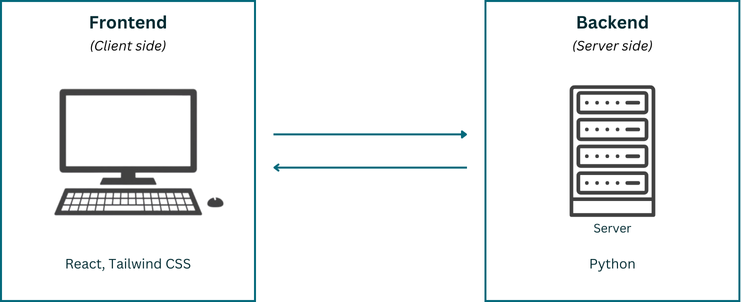
\includegraphics[scale=0.4]{imgs/simple_architecture.png}
    \caption{System Architecture. This figure shows the various components of this system, client and server components.}
    \label{fig:simple_architecture}
\end{figure}

\textbf{TO-DO}: Create a more detailed architecture on the \textit{backend} part, and the interaction between \textit{frontend} and \textit{backend}.

As we can see in Fig. \ref{fig:simple_architecture}, this system consists of two different components, \textit{backend} and \textit{frontend} components. The \textit{backend} of the system was developed in \textit{Python} and uses the \textit{FastAPI} library to build an API for our system. The frontend of the system was developed in \textit{React} and uses the \textit{Tailwind CSS} framework for styling our website. It also uses, the \textit{PyDub} library to convert an \textit{MP3} file into a \textit{WAV} file, and the \textit{Librosa} library to load the received audio data and convert them into floating point time series.

\subsection{Requirements}

To ensure the development of a robust BPM detection system, it is essential to establish a set of requirements. Our system needs to follow these requirements:

\begin{itemize}
    \item \textbf{Functional requirements}:
        \begin{itemize}
            \item The system should accept multiple file types (\textit{MP3} and \textit{WAV}).
            \item The system should allow users to upload a file via the web interface.
            \item The solution must detect \textit{BPM} of the uploaded audio file.
            \item The solution should handle changes in BPM during the duration of the song.
            \item The system should present a real-time \textit{BPM} graph while the song plays in the background. 
            \item The system should allow users to view their history of previous \textit{BPM} detections. 
        \end{itemize}
    \item \textbf{Non-Functional requirements}:
        \begin{itemize}
            \item The web interface should be intuitive and easy to navigate. 
            \item The system should be reliable by ensuring consistent \textit{BPM} detection across multiple runs of the same audio file.
        \end{itemize}
\end{itemize}

\subsection{How to use the solution?}

In Fig. \ref{fig:main_page_with_music}, you can see the main page of the system, where the user can upload any music file and see the \textit{BPM} values for every second of the song while the song is playing in the background. In addition, the user can view their history by clicking on the button in the top right corner.

\begin{figure}[h]
    \centering
    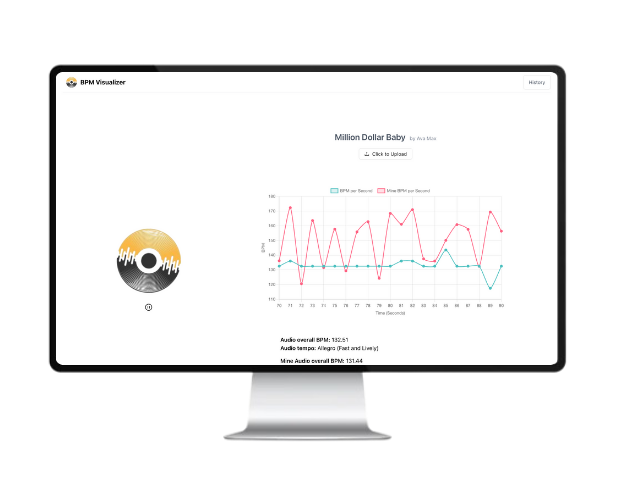
\includegraphics[scale=0.45]{imgs/main_page_with_music_with_pc_frame.png}
    \caption{Main page. This figure shows the main page of our system with the various functionalities available.}
    \label{fig:main_page_with_music}
\end{figure}

\section{Procedure}
In our solution, we implemented two approaches. The initial approach uses energy and peak detection to calculate \textit{BPM} on each sample. The second approach adopts a hybrid multi-band approach that splits the audio frequency ranges into three frequency ranges.

\subsection{Initial approach}
In the initial approach, we applied a \textbf{bandpass} filter, so that the system only focuses on frequencies that are relevant for the detection of beats (range of musical frequencies). This reduces noise and irrelevant frequencies, improving the accuracy of the system. 
Then, we divided the signal into 5 second samples. For each sample, we calculated the energy of the wave, and we smooth this energy using a uniform filter over a 100ms window to reduce noise.

In order to obtain the overall \textit{BPM} of the uploaded song, the following procedure was established:

\begin{enumerate}
    \item \textbf{File conversion}: Firstly, the file was converted from an \textit{MP3} file type into a \textit{WAV} file type by using the \textit{Fourier-Fast Transform} (\textit{FFT}) method.
    
        \begin{IEEEeqnarray}{rCl}
            x(t) = \int_{-\infty}^{\infty} x(t) * e^{-j 2\pi f t} \,dt
        \end{IEEEeqnarray}

    
    \item \textbf{Audio division}: Subsequently, the audio was splitted into 1 second samples. By splitting the audio into 1-second samples, it allows to process the audio and detect the music tempo more accurately.
    
    \item \textbf{Smooth audio sample}: For each segment, the audio segment was smooth by calculating the its energy, to ensure that the \textit{BPM} detection is based on genuine patterns rather than spontaneous artifacts or noise.

        \begin{IEEEeqnarray}{rCl}
            E(t) = |A|^2
        \end{IEEEeqnarray}

        where \(A\) is the amplitude of the signal at time \(t\).
    
    \item \textbf{Peaks detection}: Moreover, we detected significant audio peaks (by defining a peak height threshold and a minimum distance between the detected peaks).
    
    \item \textbf{\textit{BPM} calculation}: If it was detect at least 2 peaks, the \textit{BPM} is calculated based on the average interval between peaks.
    
        \begin{IEEEeqnarray}{rCl}
            BPM = \frac{60}{average\_interval}
        \end{IEEEeqnarray}

        If not at least two peaks were detected, we apply the interpolation process between the two nearest neighbours.
    
    \item \textbf{Overall song BPM}: Furthermore, we applied the \textit{DBSCAN} clustering algorithm to determine the overall BPM of a song based on the \textit{BPM} values detected for each sample. This clustering algorithm was used since it handles noise and outliers in the audio data. This clustering algorithm forms clusters based on the data density, which helps to detect the most dominant cluster in the song. And, subsequently, to detect the song's BPM by calculating the mean of the BPM values of the most dominant cluster.

        

        \begin{figure}[h]
            \centering
            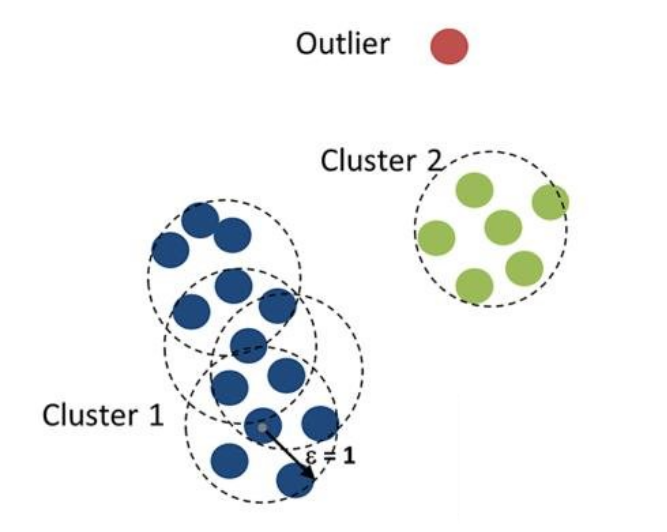
\includegraphics[scale=0.30]{imgs/DBSCAN_algorithm.png}
            \caption{\textit{DBSCAN} algorithm. Divides the values into clusters and removes outliers.}
            \label{fig:main_page_with_music}
        \end{figure}
    
        Equation~\ref{eq:centroid_calculation} is used to calculate the centroid of the cluster. The centroid value is the mean of all \textit{BPM} values that belong to the cluster.

        \begin{IEEEeqnarray}{rCl}
            \text{cluster\_centroid\_C} & = \frac{\sum\limits_{i=1}^{n} \text{BPM}_{i}}{n}
            \label{eq:centroid_calculation}
        \end{IEEEeqnarray}

    \item \textbf{Detect song \textit{tempo}}: After detecting the song \textit{BPM}, the song tempo was determine by a predefined list of \textit{BPM} ranges.

        \begin{table}[h]
            \centering
            \caption{Musical Tempo Ranges Based on BPM}
            \label{tab:tempo_ranges}
            \begin{tabular}{@{}lll@{}}
            \toprule
            Tempo Category                           & BPM Range     \\ \midrule
            \textit{Very Slow} (Below Largo)         & 0-39          \\
            \textit{Largo} (Very Slow)               & 40-60         \\
            \textit{Adagio} (Slow and Stately)       & 61-76         \\
            \textit{Andante} (Walking Pace)          & 77-108        \\
            \textit{Moderato} (Moderate)             & 109-120       \\
            \textit{Allegro} (Fast and Lively)       & 121-156       \\
            \textit{Vivace} (Lively and Fast)        & 157-176       \\
            \textit{Presto} (Very Fast)              & 177-200       \\
            \textit{Prestissimo} (Extremely Fast)    & \textgreater 201      \\ \bottomrule
            \end{tabular}
        \end{table}
    
\end{enumerate}

\subsection{Hybrid multi-band approach}
In this approach, we decided to replicate the approach studied in \textit{"Survey paper on music beat tracking
"} by Makarand Velankar. In the hybrid multi-band approach, the incoming audio is splitted into three frequency ranges. In order to obtain the overall \textit{BPM} of the uploaded song, this method took the following procedure:

\begin{enumerate}
    \item \textbf{File conversion}: Firstly, we needed to convert the uploaded file using the \textit{FFT}, similar to the initial approach.
    
    \item \textbf{Bandpass filter}: Then, the signal was divided into three frequency ranges.

        \begin{itemize}
            \item \textbf{Low-frequency range}: From 0 to 200 Hz (capturing percussive instruments).
            \item \textbf{Medium-frequency range}: From 200 to 5000 Hz (capturing melody).
            \item \textbf{High-frequency range}: Above 5000 Hz (capturing transients).
        \end{itemize}

    \item \textbf{Onset (\textit{SC}) and Transient (\textit{TD}) detection}: Detect onsets and transients in each frequency range to identify relevant rhythmic peaks. 

        \begin{itemize}
            \item \textbf{Low-band frequencies}: We used spectral-onset detections. This method was identified as a very suitable representation for tempo extraction as it tracks energy changes in the magnitude spectrum. It is effective in identifying slow onsets and rhythmic patterns.
            \item \textbf{Mid-band frequencies}: For this frequency range, we used a transient detection method. This method counts the number of bins that represent localized energy spikes while ignoring lower-amplitude noises.
            \item \textbf{High-band frequencies}: For this frequency range, we also used a transient detection method. So, even if the energies of the bins of a  transient signal are low, this method will track a new occurrence if the transient spreads over this frequency range.
        \end{itemize}

        The following formulas help to understand the detection of onsets (Equation~\ref{eq:odf}) and transients (Equation~\ref{eq:transient_1} and Equation~\ref{eq:transient_2}) on the signal.

        \begin{IEEEeqnarray}{rCl}
            ODF(t) = \max(\dv{x(t)}{t}) \quad \text{for} \quad t \in [0, \mathrm{T}]
            \label{eq:odf}
        \end{IEEEeqnarray}

        where $x(n)$ is the amplitude of the signal at time $n$, $x(n - 1)$ is the amplitude of the signal at the previous time step, and $\mathrm{T}(n)$ represents the magnitude of change (transient) between consecutive samples.

        \begin{IEEEeqnarray}{rCl}
            \mathrm{T}(n) &=& \left| x(n) - x(n - 1) \right| \label{eq:transient_1}
        \end{IEEEeqnarray}

        \begin{IEEEeqnarray}{rCl}
            \text{Transient}(n) & = &
            \begin{cases} 
                1, & \text{if } T[n] > \text{Threshold}, \\
                0, & \text{otherwise}.
            \end{cases}
            \label{eq:transient_2}
        \end{IEEEeqnarray}

        where $x(n)$ is the amplitude of the signal at time $n$, $x(n - 1)$ is the amplitude of the signal at the previous time step, and $\mathrm{T}(n)$ represents the magnitude of change (transient) between consecutive samples.
        
        

        \begin{table}[h!]
            \centering
            \caption{Proposed Hybrid Multi-band Configuration} % Caption placed before the table
            \label{table:hybrid-config} % Label immediately after caption
            \begin{tabular}{|c|c|c|}
                \hline
                \textbf{Low Freq Band} & \textbf{Middle Freq Band} & \textbf{High Freq Band} \\ \hline
                SC & TD & TD \\ \hline
            \end{tabular}
        \end{table}

    \item \textbf{Periodicity Detection method}: Succeeding the onset and transient detections, existing periodicities are calculated after getting the \textit{PeDF} in each frequency range. This detection used an autocorrelation to identify rhythmic patterns.

    \item \textbf{Combination of \textit{PeDFs}}: After having all the \textit{PeDFs} for the different frequency bands, these ranges are combined into a single unified \textit{PeDF} using weighted contributions, as we can see in Equation~\ref{eq:PeDFs_combination}.

        \begin{IEEEeqnarray}{rCl}
            \mathrm{Combined\ PeDF} &=& w_{low} \cdot \mathrm{PeDF}_{low} \quad + \nonumber \\
            && w_{med} \cdot \mathrm{PeDF}_{med} \quad + \nonumber \\ 
            && w_{high} \cdot \mathrm{PeDF}_{high}
            \label{eq:PeDFs_combination}
        \end{IEEEeqnarray}

    \item \textbf{Detection of peaks}: Finally, after calculating the combined \textit{PeDF}, we needed to find relevant peaks (in our study we used the mean of the values of the combined \textit{PeDF} to represent the heigh threshold for peak detection).

    \item \textbf{BPM calculation}: Similar to the first method, if at least 2 peaks were detected, the \textit{BPM} is calculated based on the average interval between peaks.

    \item \textbf{Overall song BPM}: Finally, the \textit{tempo} is defined based on the \textit{BPM} obtained from the previous step.
        
\end{enumerate}

\section{Program solution evaluation}

In order to evaluate our program solution, we evaluated the transparency, flexibility, reliability, performance and scalability. 

\subsection{Transparency}

In order to measure the transparency of our solution, we used the \textit{Python} library \textit{Pylint} for the backend \textit{API}, and the library \textit{ESLint} for the frontend.
For the backend score, the library \textit{Pylint} was used to check the code quality of the system. The score obtained was 6.36 out of 10.
For the frontend score, the library \textit{ESLint} was used to analyse static code. The score obtained was 

\section{Future work}

In order to improve the BPM detection pipeline, I want to use the approach described in the paper "Survey paper on music beat tracking" by \textit{Makarand Velankar} \cite{approachByMakarandVelankar}. In this approach, they divided the frequency spectrum into 3 ranges (\textit{Low-frequency band}, \textit{Middle-frequency band} and \textit{high frequency band}, while using onset and transient detectors to determine the song's \textit{Periodicity Detection Function} (\textit{PeDF}) and then get the overall song's BPM. This approach will allow for more precise and reliable beat tracking and tempo detection in songs.

\section{Conclusion}

This project demonstrates the development and implementation of a sophisticated system that accurately determines the beats per minute (\textit{BPM}) of the uploaded song.

The integration of the \textit{BPM} overtime graph significantly enhanced the user interface, offering a dynamic and interactive experience.

In conclusion, the current state of this project meets the initial proposed plan. The future work described will be done until the end of the project development phase, and some user interface will be enhanced to improve user's experience on our system.


\bibliography{report}


\end{document}